% ============================================================
%  sec05_06a.tex
%  §5 Hochschild 上同调与 $A_\infty$-结构的分类（原文 pp.21–24）
%  §6 $\Lambda_t$ 上椭圆曲线的镜像对称，含 6.1 代数 $Q$
%     （原文 pp.24–28，止于 p.29 “6.2. The derived category of an elliptic curve” 标题之前）
%  原文：Homological Mirror Symmetry for Elliptic Curves（2013-04-25）
%  说明：文献引用沿用原文编号 [n]；跨节引用使用 GUIDE §6.5 登记的标签 key。
% ============================================================

\section{\texorpdfstring{Hochschild 上同调与 $A_\infty$-结构的分类}{Hochschild 上同调与 A∞-结构的分类}}\label{sec:hoch}

\begin{keytakeaways}
  \item \textbf{数学工具}：把 $A_\infty$-代数重新表述为约化余张量余代数 $\bar T(SA)$ 上次数为一的余微分 $b$；$A_\infty$-方程恰是 $b^2=0$，$A_\infty$-态射恰是与 $b$ 交换的余代数态射。
  \item \textbf{代数机制}：Hochschild 复形 $CC^{m,n}=\Hom_k(A^{\otimes m},SA(n))$ 上的微分是超 Lie 括号 $D=[b,\cdot]$，因此 $HH^{m,n}(A)\simeq\Ext^m_{A\otimes A^{op}}(A,A(n))$。
  \item \textbf{核心结论}：延拓给定乘法的 $A_\infty$-结构，其规范等价类的自由度逐阶由 $HH^{d,2-d}(A)$ 控制；若这些群除 $d=R$ 外全为零、在 $d=R$ 处一维，则至多差一个障碍类（定理 \ref{thm:5.3}）。
  \item \textbf{几何图像}：$HH^{\bullet,2-\bullet}$ 上有一个自然的重标度作用 $\epsilon$，它把障碍类按 $\tilde\epsilon^{d-2}$ 缩放；下一节将看到，这正是镜像映射把 $a_4,a_6$ 与 Weierstrass 系数 $a,b$ 对齐的代数根源。
\end{keytakeaways}

本节说明如何用 Hochschild 上同调对极小的 $A_\infty$-结构进行分类。第一小节用分次余代数重新解释 $A_\infty$-代数，这部分材料在 [9, 3.6] 中有最简洁的总结。第二小节定义 Hochschild 上同调并说明它的一些性质，其中大部分材料可在 [5] 以及 [19, 第 3 节] 中找到。

\subsection{\texorpdfstring{$A_\infty$-结构与余代数余微分}{A∞-结构与余代数余微分}}\label{subsec:coalgebra}

我们先以一种不那么“就事论事”的方式重新解释 $A_\infty$-方程。为此回忆：\emph{分次余代数}是分次向量空间 $V$ 连同余乘法 $\Delta:V\to V\otimes V$，满足某种与代数定义相对偶的“结合性条件”；\emph{次数为 $d$ 的余导子}是 $\Hom(V,V(d))$ 中的一个元素，满足某种与代数上导子定义相对偶的关系；最后，余代数态射的概念同样按显然的方式定义。我们指出：$\Delta$ 与余代数态射都自动是次数为零的。

% [Tutor Note: 此处“对偶”不是把箭头简单地反向：分次情形下取对偶 $V\mapsto V^*=\bigoplus_n\Hom(V_n,k)$ 会翻转次数并引入 Koszul 符号，所以“与结合性相对偶的条件”是一个带符号的多重线性恒等式，而不是把 $\mu\circ(\mu\otimes1)=\mu\circ(1\otimes\mu)$ 的字面转写。本节让 $\Delta$ 与余代数态射自动为次数零，全部符号都推迟到 $A_\infty$ 方程、Hochschild 微分与 Lie 括号里出现，这是最容易在读第二遍时搞混的地方。]

我们主要的余代数例子如下。设 $V$ 是分次向量空间，则 $V$ 上的\emph{约化余张量余代数}（reduced cotensor coalgebra）为
\[
\bar TV=\bigoplus_{n>0}V^{\otimes n}.
\]
以下把 $v_1\otimes\cdots\otimes v_n$ 记作 $v_1\ldots v_n$，并给 $\bar TV$ 赋分次 $|v_1\ldots v_n|=|v_1|+\cdots+|v_n|$。记 $\bar T^nV=V^{\otimes n}$，视之为 $\bar TV$ 的子空间。余乘法由
\[
\Delta(v_1\ldots v_n)=\sum_{k=1}^{n}(v_1\ldots v_k)\otimes(v_{k+1}\ldots v_n)
\]
定义。

% [Tutor Note: $\Delta$ 的公式里 $k$ 遍历所有可能的切分位置；$k=n$ 时右侧第二因子是空词。约化余张量余代数通常把空词当作单位元 $1$ 并令 $\Delta(1)=0$，原文未明说但后文所有公式都不涉及这一项；若在别的文献中看到 $\Delta(v_1)=v_1\otimes1+1\otimes v_1$，那是非约化版本，切勿与本节的 $\Delta$ 混用。]

这个余代数在许多方面表现得“对偶于”通常的张量代数。它的性质总结为下述命题，其证明是一个容易的练习。

\begin{proposition}\label{prop:5.1}
设 $V$ 与 $W$ 是分次向量空间。记 $\pi:\bar TV\to V$ 为到第一个直和项的投影。对任意分次向量空间 $U$ 与线性映射 $f:U\to\bar TV$，把 $\pi_*(f)$ 记作复合 $\pi\circ f$。
\begin{enumerate}
  \item 映射
  \[
  \{\text{$\bar TV\to\bar TV$ 上次数为 $d$ 的余导子}\}\xrightarrow{\ \pi_*\ }\Hom_k(\bar TV,V(d))=\prod_{n>0}\Hom_k(V^{\otimes n},V(d))
  \]
  是双射；其逆映射把 $(b_i)\in\prod_{n>0}\Hom_k(V^{\otimes n},V(d))$ 送到 $b$，其中
  \[
  b|_{\bar T^nV}=\sum_{a+b+c=n}1^{\otimes a}\otimes b_i\otimes 1^{\otimes b}.
  \]
  \item 映射
  \[
  \{\text{$\bar TV\to\bar TW$ 的余代数态射}\}\xrightarrow{\ \pi_*\ }\Hom_k(\bar TV,W)=\prod_{n>0}\Hom_k(V^{\otimes n},W)
  \]
  是双射；其逆映射把 $(f_i)\in\prod_{n>0}\Hom_k(V^{\otimes n},W)$ 送到 $f$，其中
  \[
  f|_{\bar T^nV}=\sum_{r,\ a_1+\cdots+a_r=n}f_{a_1}\otimes\cdots\otimes f_{a_r}.
  \]
\end{enumerate}
\end{proposition}

% [Tutor Note: 命题 5.1 的“容易练习”实质上要做两件事：(i) 用余张量余代数的泛性质验证“余导子/余代数态射”与“分量族 $(b_i)$/$(f_i)$”一一对应；(ii) 验证由所示公式拼出的 $b$ 确实满足余导子条件 $\Delta b=(b\otimes1+1\otimes b)\Delta$。关键机制是：$\Delta$ 把长度 $n$ 的词拆成长度 $k$ 与 $n-k$ 的两段，而 $b$ 只作用在其中一段上，故求和遍历该连续子词的全部位置。]

% [Tutor Note: 原文疑误：$b|_{\bar T^nV}=\sum_{a+b+c=n}1^{\otimes a}\otimes b_i\otimes1^{\otimes b}$ 的指标不自洽——和式用了 $a,b,c$ 三个指标，但右侧只出现 $1^{\otimes a}$、$b_i$、$1^{\otimes b}$，$c$ 与 $i$ 都没有被和式约束。按标准公式应为 $\sum_{a+i+c=n}1^{\otimes a}\otimes b_i\otimes1^{\otimes c}$（即分量 $b_i$ 作用在长度 $i$ 的连续子词上，左右各固定 $a$、$c$ 个因子）。译文保留原文写法，使用时请按标准公式理解。]

以下我们也把 $\pi_*(f)$ 在 $\bar T^iV$ 上的限制记作 $\pi_*(f)_i\in\Hom(V^{\otimes i},V(d))$。

我们引入这些余代数的主要原因是它们与 $A_\infty$-代数的联系。下述命题同样只是把定义写开的一个容易练习。对分次向量空间 $V$，记 $SV$ 为分次向量空间 $V(1)$，$s:V\to SV$ 为自然的（次数 $-1$ 的）\emph{平移映射}。

\begin{proposition}\label{prop:5.2}
\begin{enumerate}
  \item 设 $A$ 是分次向量空间。$A$ 上的 $A_\infty$-结构与 $\bar T(SA)$ 上次数为一的余微分是同一回事。确切地说，给定余微分 $(b_i)\in\prod_{n>0}\Hom_k((SA)^{\otimes n},SA(1))$，由
  \[
  m_i=s^{-1}b_is^{\otimes i}\in\Hom_k(A^{\otimes n},A(2-i))
  \]
  给出的映射 $m_i$ 定义 $A_\infty$-结构，当且仅当 $b^2=0$。
  \item 设 $A$ 与 $B$ 是 $A_\infty$-代数，相应的余导子为 $b_A$ 与 $b_B$。则 $A_\infty$-态射 $A\to B$ 与满足 $fb_A=b_Bf$ 的余代数态射 $f:\bar T(SA)\to\bar T(SB)$ 是同一回事。
\end{enumerate}
\end{proposition}

% [Tutor Note: 符号易错：$s$ 的次数为 $-1$，故 $\deg s^{-1}=+1$、$\deg s^{\otimes i}=-i$；又 $\deg b_i=1$，于是 $\deg m_i=(+1)+1-i=2-i$，这正是 $A_\infty$-结构映射 $m_i:A^{\otimes i}\to A(2-i)$ 的标准次数（$m_2$ 次数 $0$，$m_3$ 次数 $-1$，依此类推）。若把 $s$ 误当成次数 $+1$，所有次数都会整体平移，$A_\infty$ 方程的符号也会随之改变。]

% [Tutor Note: 原文疑误：命题 5.2 中 $m_i=s^{-1}b_is^{\otimes i}$ 的陪域写作 $\Hom_k(A^{\otimes n},A(2-i))$，但 $m_i$ 取 $i$ 个输入，应为 $\Hom_k(A^{\otimes i},A(2-i))$。这一句里乘积指标 $n$ 与分量指标 $i$ 混用了（$(b_i)\in\prod_{n>0}\Hom_k((SA)^{\otimes n},SA(1))$ 亦如此）。译文保留原文写法。]

本节余下部分固定一个分次向量空间 $A$。记
\[
C^{m,n}=\Hom_k((SA)^{\otimes m},SA(n)),\qquad C^n=\Hom_k(\bar T(SA),SA(n))\simeq\prod_r C^{r,n}.
\]
上述命题允许我们把 $C^n$ 看作 $\bar T(SA)$ 上余导子的空间。对分次余导子 $b_1$ 与 $b_2$，记
\[
[b_1,b_2]=b_1b_2-(-1)^{|b_1||b_2|}b_2b_1,
\]
并称之为（超）\emph{Lie 括号}。易于验证它满足\emph{分次 Jacobi 恒等式}
\begin{equation}\label{eq:hoch-jacobi}
(-1)^{|x||z|}[x,[y,z]]+(-1)^{|y||x|}[y,[z,x]]+(-1)^{|z||y|}[z,[x,y]]=0 .
\end{equation}
还可验证 Lie 括号与分次相容，即 $[C^{m,n},C^{p,q}]\subset C^{m+p-1,n+q}$。

% [Tutor Note: 式 \eqref{eq:hoch-jacobi} 的 Koszul 符号极易抄错：三项的符号 $(-1)^{|x||z|}$、$(-1)^{|y||x|}$、$(-1)^{|z||y|}$ 恰好是把对应的第一个元素移到最左端所需的符号，因此三项是同一个式子的循环置换。注意本文的括号是 $[b_1,b_2]=b_1b_2-(-1)^{|b_1||b_2|}b_2b_1$；当 $b_1,b_2$ 均为奇（例如两个次数一的余导子）时它就是反对易子 $b_1b_2+b_2b_1$。]

\subsection{Hochschild 上同调}\label{subsec:hoch-cohomology}

\begin{definition*}
设 $A$ 是分次向量空间。记
\[
CC^{m,n}=CC^{m,n}(A)=\Hom_k(A^{\otimes m},SA(n))
\]
为 Hochschild 链空间（Hochschild chain spaces），并记 $CC^n=\prod_{p+q=n}CC^{p,q}$。
\end{definition*}

借助 $s:A\to SA$，有同构（作为分次向量空间）$CC^{m,n}\simeq C^{m,m+n-1}$ 与 $CC^n\simeq C^n$。这把超 Lie 结构移植到 $CC^{\bullet,\bullet}$ 上。

% [Tutor Note: 这两个同构是由 $s$ 诱导的：把 $\Hom_k(A^{\otimes m},SA(n))$ 中的元素 $x$ 的两侧分别乘以 $s$ 与 $(s^{-1})^{\otimes m}$，即 $x\mapsto sx(s^{-1})^{\otimes m}$，就得到 $\Hom_k((SA)^{\otimes m},SA(\cdot))$ 中的元素，第二个指标恰好差 $m-1$。验证时把 $|s|=-1$ 逐项代入，是检查上述“$\simeq$”是否抄对的唯一稳妥办法。]

现设 $A$ 是分次代数。回忆这只是 $A_\infty$-代数的特例：$m_i=0$（$i\neq2$），因此命题 \ref{prop:5.2} 给出次数为一的余微分 $b\in CC^{2,0}$。对 $x\in CC^{m,n}$，定义 \emph{Hochschild 微分} $D(x)=[b,x]$。有
\[
D(CC^{m,n})\simeq[b,C^{m,m+n-1}]\subset C^{m+1,m+n}\simeq CC^{m+1,n}.
\]
分次 Jacobi 恒等式 \eqref{eq:hoch-jacobi} 说明 $D$ 确实是微分，且满足\emph{分次 Leibniz 法则}。

% [Tutor Note: 原文此处把 "Leibniz" 误排为 "Leinbniz"（p.23），译文按正确拼写处理。]

% [Tutor Note: 注意 $D=[b,\cdot]$ 是双分次 $(1,0)$ 的：它把第一个指标（输入因子个数，对应 $\Ext$ 的次数）加一，而第二个指标 $n$（内部分次，对应系数平移 $A(n)$）保持不变。因此对每个固定的 $n$，$CC^{\bullet,n}$ 各自是一个复形——上同调 $HH^{m,n}$ 的双分次结构即由此而来，读后面 $\Ext^m_{A\otimes A^{op}}(A,A(n))$ 时不要漏掉这个 $n$。]

\begin{definition*}
$A$ 的\emph{双分次 Hochschild 上同调}（bigraded Hochschild cohomology）是 $CC^{\bullet,n}(A)$ 关于 $D$ 的上同调 $HH^{m,n}(A)$。
\end{definition*}

一个重要观察是：如此定义的 Hochschild 微分恰好与 $A$ 的上同调 bar 复形上的微分一致。由此得到重要公式（其中 $A^{op}$ 表示 $A$ 的反分次代数）
\[
HH^{m,n}(A)\simeq\Ext^m_{A\otimes A^{op}}(A,A(n)).
\]

% [Tutor Note: 这里省略的关键一步是：bar 复形与 Hochschild 复形只差一个由 $s$ 给出的分次向量空间同构，而 bar 复形的微分正是 $[b,\cdot]$。标准参考见 [19, §3]（Seidel）或 [5]。要建立 $\Ext$ 的解释，还需注意 $\Ext^\bullet_{A\otimes A^{op}}(A,A(n))$ 由 $A^e=A\otimes A^{op}$ 的投射消解计算，而 $A$ 上的 $n$-上链 $A^{\otimes n}\to A$ 与 $A^e$-模同态之间有标准对应。]

我们现在关心如下问题。称 $A$ 上的 $A_\infty$-结构 $(m_i)$（等价地，余微分 $(d_i)$）\emph{延拓乘法}，若 $m_1=0$ 且 $m_2$ 是来自 $A$ 的乘法（等价地，$d_1=0$ 且 $d_2=b$）。回忆第 \ref{sec:ainf} 节关于同调微扰论的内容：形式微分同胚由一族 $f_i:A^{\otimes i}\to A(1-i)$ 给出，其中 $f_1$ 可逆。若 $f_1=1$，则称之为\emph{规范变换}（gauge transformation）。注意：形式微分同胚与余代数自同构 $\Phi:\bar T(SA)\to\bar T(SA)$ 是同一回事（由命题 \ref{prop:5.2} 第 (2) 部分与命题 \ref{prop:2.2}）。于是可定义余微分 $\Phi^*(d)=\Phi^{-1}d\Phi$，它给出 $A$ 上新的 $A_\infty$-结构。若 $\Phi$ 来自规范变换，则称这些 $A_\infty$-结构\emph{规范等价}。

我们希望把 $A$ 上延拓乘法的 $A_\infty$-结构按规范等价分类。下述定理同样只是把定义写开的一个练习。

\begin{theorem}\label{thm:5.3}
设 $A$ 是结合分次代数，$d$ 与 $d'$ 是延拓乘法的次数为一的余微分。
\begin{enumerate}
  \item 设 $x\in\Hom_k((SA)^{\otimes r},SA)$。若 $\Phi$ 表示由
  \[
  \pi_*(\Phi)_n=\begin{cases}1, & n=1,\\ x, & n=r,\\ 0, & \text{其他}\end{cases}
  \]
  给定的形式微分同胚，则
  \[
  \Phi^*(d)_n=\begin{cases}b_k, & n\le r,\\ b_{r+1}+D(x), & n=r+1.\end{cases}
  \]
  \item 设存在整数 $r\ge2$ 与 $0\le s\le r-2$，使得
  \[
  \begin{aligned}
  \pi_*(d)_n&=\pi_*(d')_n &&\text{对 } n\le r,\\
  \pi_*(d)_{2+n}&=0 &&\text{对 } 0<n\le s.
  \end{aligned}
  \]
  则 $\pi_*(d-d')_n\in CC^{n,2-n}$ 对 $r<n\le r+s+1$ 是 Hochschild 上链。
\end{enumerate}
\end{theorem}

% [Tutor Note: 后文（p.25）“出于纯形式的理由”指的就是下面的 $\epsilon$ 作用：$\epsilon$ 是分次代数自同构，故它作用在 $d_i$ 上只按次数缩放，这正是 $\epsilon^*(d)_i=\tilde\epsilon^{i-2}d_i$ 的内容。注意定理 \ref{thm:5.3} 第 (1) 部分只处理“单个分量 $b_{r+1}$ 加上一个上链”的情形，迭代使用它就能逐阶消去 $m_d$；第 (2) 部分则给出两个结构在下一次障碍出现前的一致程度。]

% [Tutor Note: 原文疑误：定理 5.3 第 (1) 部分写作 $\Phi^*(d)_n=b_k$（$n\le r$）。当 $n\le r$ 时 $\pi_*(\Phi)_n$ 只在 $n=1,r$ 非零，扰动尚未波及第 $n$ 个分量，故应保持不变，即 $b_n$。译文保留原文写法（下标 $k$ 在式中无定义）。]

这是一个相当有效的工具。例如，设 $HH^{d,2-d}(A)=0$ 对 $d>2$、$d\neq R$ 成立，且 $\dim_kHH^{R,2-R}=1$。若 $(m_i)$ 是延拓乘法的 $A_\infty$-结构，则可对 $d'=b$、$r=2$ 应用定理第 (2) 部分，断言 $m_3$ 定义一个上链。若设 $R>3$，从而 $HH^{3,-1}(A)=0$，则可应用定理第 (1) 部分找到规范等价的 $A_\infty$-结构使 $m_3=0$。于是我们能平凡化直到 $m_R$ 的所有高阶乘法，此时得到障碍类 $[m_R]\in HH^{R,2-R}(A)$。若 $[m_R]=0$，便可继续平凡化，从而说明该 $A_\infty$-结构是形式的。即便不然，若 $(m'_i)$ 是另一个平凡化到 $R-1$ 阶的 $A_\infty$-结构，且 $[m_R]=[m'_R]$，我们就能对相应于 $(m'_i)$ 的 $d'$ 继续应用定理，从而说明这两个 $A_\infty$-结构实际上规范等价。因此延拓乘法的 $A_\infty$-结构（在规范等价意义下）至多构成一维族。

% [Tutor Note: 这一段是形变理论的标准论证（逐阶消去 + 障碍类）：$m_d$ 的次数为 $2-d$，故它天然落在 $HH^{d,2-d}$ 中；条件“除 $d=R$ 外全为零”意味着形变问题在 $R$ 阶之前无障碍、在 $R$ 阶恰有一个一维障碍。物理上这对应模空间在相应阶数上是光滑的、只有一个方向被挡住。]

若不只考虑规范等价，而允许所有 $A_\infty$-同构，则还能做得更好。事实上，对 $\tilde\epsilon\in k^{\times}$，由 $\epsilon_1:A\to A$，$x\mapsto\tilde\epsilon^{|x|}x$ 与 $\epsilon_n=0$（其余 $n$）给定的形式微分同胚 $\epsilon$ 具有性质
\[
\epsilon^*(d)_i=\epsilon^{i-2}d_i .
\]

% [Tutor Note: 原文疑误：此式右侧的 $\epsilon$ 应为标量 $\tilde\epsilon$，即 $\tilde\epsilon^{i-2}d_i$。若照字面理解，$\epsilon$ 是形式微分同胚（一族映射），$\epsilon^{i-2}$ 无意义。译文保留原文写法。]

现设 $k$ 代数闭。则在上述情形中（其中 $HH^{2}(A)$ 是一维的），延拓乘法的 $A_\infty$-结构至多有两个同构类：形式的（其中 $m_i=0$ 对所有 $i>2$），以及（若存在）另一个结构，其中 $m_i=0$ 对 $i<r$ 但 $[m_r]\neq0\in HH^{r,2-r}(A)$。确切地说，给定任意两个平凡化到 $r-1$ 阶的非形式 $A_\infty$-结构，都能找到 $\tilde\epsilon$ 使 $[\epsilon^*(m)_r]=[m'_r]$，再由上面的论证即知这些 $A_\infty$-结构同构。

% [Tutor Note: 原文疑误（待核）：此处写“$HH^2(A)$ 是一维的”，但本段前述设定是 $\dim_kHH^{R,2-R}(A)=1$。按上下文，起作用的应是 $HH^{R,2-R}(A)$（若把双分次的总次数记为 $m+n$，则 $HH^{2}(A)$ 也许是它的简写）；此处与 $HH^2$ 的通常含义（总次数为 $2$ 的部分）并不一致，请以 $HH^{R,2-R}$ 为准。译文保留原文写法。]

% [Tutor Note: $\epsilon$ 的作用就是 $A_\infty$-代数上的 $\mathbb{G}_m$ 重标度：它把 $m_i$ 乘上 $\tilde\epsilon^{i-2}$。这个作用在下一节（p.25）会被明确称为 $HH^{*,2-*}$ 上的自然 $\mathbb{G}_m$ 作用，是理解 $a_4,a_6$ 为何必须与 $a,b$ 同次数的关键。]

\section{\texorpdfstring{$\Lambda_t$ 上椭圆曲线的镜像对称}{Λ_t 上椭圆曲线的镜像对称}}\label{sec:mirror}

\begin{keytakeaways}
  \item \textbf{物理/几何图像}：镜像对称把平坦环面 $T$ 的辛几何（A-模型）与椭圆曲线 $E$ 的复几何（B-模型）对应起来；$T$ 的两条标准经线 $A,B$ 应当对应 $E$ 上的两个线丛 $\mathcal{O}$ 与 $\mathcal{O}(P)$。
  \item \textbf{数学工具}：先在一般特征零域 $k$ 上算出关系代数 $\mathcal{Q}$ 的上同调代数 $Q$ 的 Hochschild 上同调（命题 \ref{prop:6.2}），再用定理 \ref{thm:5.3} 的控制把任意 $A_\infty$-结构逐阶平凡化。
  \item \textbf{核心结论}：存在椭圆曲线 $E/\Lambda_t$ 与 $A_\infty$-范畴的拟等价 $D^\pi\Fuk(T)\to D_\infty(E)$（定理 \ref{thm:6.1}）；$Q$ 的 $HH^{d,2-d}$ 仅在 $d=6,8$ 时为一维。
  \item \textbf{关键机制}：Weierstrass 族 $\mathcal{X}\to\mathbb{A}^2$ 连同 $\mathbb{G}_m$ 作用使平凡化程序对所有（含奇异）纤维统一进行；所得 $a_4(a,b)$、$a_6(a,b)$ 与 $a,b$ 同次数，故最终可取 $a_4=a$、$a_6=b$。
\end{keytakeaways}

现在我们准备陈述并证明椭圆曲线的同调镜像对称。我们将在特征为零的代数闭域 $\Lambda_t$ 上工作。记 $T$ 为带标准辛结构的平坦环面，其 Maslov 覆盖来自 $\Delta$ 的标准（全纯）平凡化（见 \ref{subsec:maslov} 小节）。本节的目标是证明下述定理：

% [Tutor Note: $\Lambda_t$ 是复数域上的万有 Novikov 域（universal Novikov field）：其元素是形式级数 $\sum_{n>0}a_nt^{b_n}$，其中 $a_n\in\mathbb{C}$、$b_n\in\mathbb{R}$ 且 $b_n\to\infty$（见原文 §1 的记号约定与 4.4 小节）。几何上每个全纯多边形按面积给出权重 $t^{\int u^*\omega}$，所以 $k=\Lambda_t$ 时 Floer 代数记住辛面积。本文的策略是：先在任意特征零域 $k$ 上做代数几何与 Hochschild 计算，最后特殊化到 $k=\Lambda_t$——这样“抽象 HMS”与“具体镜像映射（求 $E$ 的 $j$-不变量）”就分离开了。]

\begin{theorem}\label{thm:6.1}
存在 $\Lambda_t$ 上的椭圆曲线 $E$，以及 $A_\infty$-范畴之间的拟等价
\[
D^\pi\Fuk(T)\to D_\infty(E).
\]
\end{theorem}

% [Tutor Note: 记号 $D^\pi\Fuk(T)$ 中的上标 $\pi$ 表示对 Fukaya 范畴作幂等完备化（split-closure，即 Karoubi 完备化）后再取导出范畴；若去掉 $\pi$，范畴的生成性质会不同，阅读时不要把它当作装饰性上标。]

我们将采用引言中勾勒的证明方法。如前所说，这基本上是把 [19] 中发展的策略应用到一维情形。具体地说，我们将在 \ref{subsec:generation} 小节中证明 $T$ 的两条标准经线 $A$ 与 $B$ 分裂生成 $\Fuk(T)$（从而当然也分裂生成 $D^\pi\Fuk(T)$）。于是需要研究关系 $A_\infty$-代数 $\mathcal{Q}=\Hom_{D^\pi\Fuk(T)}(A\oplus B,A\oplus B)$。我们把它的上同调代数记作 $Q=H(\mathcal{Q})$。

在 \ref{subsec:algebra-Q} 小节中我们将说明如何计算它的 Hochschild 上同调。那里我们在任意特征为零的域 $k$ 上工作。特别地，我们将证明
\[
HH^{d,2-d}(Q)=\begin{cases}k, & d=6,8,\\ 0, & d>2,\ d\neq6,8.\end{cases}
\]
关于 Hochschild 上同调与 $A_\infty$-结构之间关系的定理 \ref{thm:5.3}，连同定理 \ref{thm:2.1} 的同调微扰论，现在给出如下结论：对任意上同调代数为 $Q$ 的 $A_\infty$-代数 $\mathcal{Q}'$，都能找到一个拟同构的 $A_\infty$-代数 $(Q,(m_d))$，其中 $m_1=0$、$m_2$ 是 $Q$ 上的乘法，并且 $m_d=0$ 对 $d=3,4,5,7$；此外 $m_6$ 与 $m_8$ 将成为上链，给出元素 $a_4(\mathcal{Q}')\in HH^{6,-4}(Q)$ 与 $a_6(\mathcal{Q}')\in HH^{8,-6}(Q)$。注意：尽管我们使用函数记号 $a_i(\mathcal{Q}')$，这些上同类先验地依赖于我们在平凡化 $A_\infty$-结构时所作的选择，而不只依赖于 $\mathcal{Q}'$。然而定理 \ref{thm:5.3} 确实蕴含：若 $\mathcal{Q}''$ 是另一个这样的 $A_\infty$-代数，且最终得到 $a_4(\mathcal{Q}')=a_4(\mathcal{Q}'')$ 与 $a_6(\mathcal{Q}')=a_6(\mathcal{Q}'')$，则 $\mathcal{Q}'$ 与 $\mathcal{Q}''$ 拟同构。

% [Tutor Note: 这是全文最微妙的一处逻辑：$a_4,a_6$ 是“先选平凡化、再读出上同调类”，所以它们不是 $\mathcal{Q}'$ 的不变量，而是依赖于选择的数据；定理 5.3 保证的是“两个结构若读出相同的 $a_4,a_6$ 则拟同构”这一单向陈述（更强的、与选择无关的结论见 [11]，作者明说此处不需要）。阅读时切勿把 $a_i$ 当作函子。]

现在我们转向镜像对称的代数几何一侧。在下一小节中，我们将在任意特征为零的代数闭域上工作。关于曲线导出范畴生成元的定理 \ref{thm:3.3} 立即蕴含：对任意椭圆曲线 $E$ 与任意（闭）点 $P\in E$，两个层 $\mathcal{O}$ 与 $\mathcal{O}(P)$ 分裂生成 $D_\infty(E)$。关系代数的上同调代数，即 $\Ext^{*}(\mathcal{O}\oplus\mathcal{O}(P),\mathcal{O}\oplus\mathcal{O}(P))$，容易计算，并且可以验证它与 $Q$ 一致。

接下来我们转向 Lekili 与 Perutz [11] 的关键洞见。具体地说，我们考虑整个 Weierstrass 族
\[
\mathcal{X}=\{X_0X_2^2=X_1^3+aX_0^2X_1+bX_0^3\}\subset\mathbb{P}^2\times\mathbb{A}^2\to\mathbb{A}^2 .
\]
当光滑时，纤维 $E_{a,b}$ 是椭圆曲线；并且它们穷尽 $k$ 上所有椭圆曲线。群 $\mathbb{G}_m$ 以自然方式作用在 $\mathcal{X}$ 上（通过 Weierstrass 重参数化 $x\mapsto u^2x$ 与 $y\mapsto u^3y$）。我们将证明：关系 $A_\infty$-代数上的平凡化程序可以对所有 $E_{a,b}$（包括奇异的！）统一地执行。于是得到类 $a_4(a,b)\in HH^{6,-4}(Q)$ 与 $a_6(a,b)\in HH^{8,-6}(Q)$，它们多项式地依赖于 $a,b$，并且与 $\mathbb{G}_m$ 的作用相容（回忆第 \ref{subsec:hoch-cohomology} 小节末尾：$HH^{*,2-*}$ 也带有自然的 $\mathbb{G}_m$ 作用）。由此可以说明（出于纯形式的理由）：适当选取一组基后，有 $a_4(a,b)=a$ 与 $a_6(a,b)=b$。特别地，（可能奇异的）Weierstrass 三次曲线给出 $Q$ 上所有可能的 $A_\infty$-结构。

% [Tutor Note: 几何直观：$\mathcal{X}\to\mathbb{A}^2$ 的判别式（相差一个非零常数）为 $4a^3+27b^2$；$4a^3+27b^2\neq0$ 时 $E_{a,b}$ 光滑，等于 $0$ 时为节点或尖点三次曲线。作者特意强调“包括奇异的”，因为 Lekili–Perutz 方法把整个 $A_\infty$ 结构族看成 $\mathbb{A}^2$ 上的代数族、而非逐条曲线处理，这样障碍类 $a_4,a_6$ 就是 $\mathbb{A}^2$ 上的多项式，奇异性不构成例外。]

% [Tutor Note: $\mathbb{G}_m$ 作用 $(x,y)\mapsto(u^2x,u^3y)$ 把 $(a,b)$ 送到 $(u^4a,u^6b)$，因此 $a_4$ 与 $a_6$ 必须分别是 $a$（次数 4）与 $b$（次数 6）的倍式；由于一维性，倍数只能是常数。这就是“适当选基后 $a_4=a$、$a_6=b$”的几何根源——不是计算巧合，而是等变性强制的结果。]

一个重要观察是：给定椭圆曲线的导出范畴 $D_\infty$ 与两个生成元 $\mathcal{O}$ 与 $\mathcal{O}(P)$，我们实际上可以重构出曲线 $E$。这是因为环 $\bigoplus_n\Hom_{H^0D_\infty}(\mathcal{O},\mathcal{O}(3nP))$ 正是 $E$ 的某个嵌入的射影坐标环。可以把该环辨认为命题 \ref{prop:2.6} 中考虑的那种形式（某些扭变函子的不变环），因此它实际上是 $D_\infty$ 的拟等价类的不变量。

综合这些想法可得到重要的重构定理 \ref{thm:6.4}，它是本文所证明的代数几何与同调代数结果的核心。

应当提到：实际上类 $a_4$ 与 $a_6$（在确切的意义下）与所作的选择无关。这在 [11] 中已有证明，但我们这里不需要如此强的结论。

我们终于可以转向辛几何一侧。在 \ref{subsec:generation} 小节中，我们将大量使用定理 \ref{thm:4.2} 中陈述的 Fukaya 范畴的性质。利用 Dehn 扭转与代数扭转的等同，以及定理 \ref{thm:2.7} 关于用扭变函子判定生成元的准则，我们证明两条标准经线 $A$ 与 $B$ 确实是 $D^\pi\Fuk(T)$ 的分裂生成元。随后我们通过计数（退化的）多边形来计算关系 $A_\infty$-代数 $\mathcal{Q}$ 的上同调代数。结果表明它与 $Q$ 一致，正如所断言。把我们的代数工作特殊化到 $k=\Lambda_t$，就完成了镜像对称的抽象证明。

剩下的问题是利用重构定理 \ref{thm:6.4} 确定 $\Lambda_t$ 上究竟哪条椭圆曲线是 $T$ 的镜像（特别地，排除镜像为奇异曲线的可能性）。这将在下一节处理。本节余下部分用于补全上面勾勒的抽象镜像对称证明的细节。

最后一点导引性说明。我们所说的一切本来都可以照原样成立。然而，若把两条标准经线 $A$ 与 $B$ 不认同为层 $\mathcal{O}$ 与 $\mathcal{O}(P)$、而是认同为 $\mathcal{O}$ 与 $\mathcal{O}/P$，镜像对应会变得最为自然。事实上，$D_\infty(E)$ 存在一个自同构，它固定 $\mathcal{O}$ 并把 $\mathcal{O}(P)$ 与 $\mathcal{O}/P$ 互换。我们之所以更愿意用 $\mathcal{O}(P)$ 而不是 $\mathcal{O}/P$ 来工作，纯粹是技术上的方便（前者是线丛）。

我们将在后面证明 $\mathcal{O}(P)=T_{\mathcal{O}/P}(\mathcal{O})$。因此在“正确的”镜像对应下，$\mathcal{O}(P)$ 的镜像是 $B'=\tau_B(A)$，这是一条斜率为 $\pi/4$ 的直线。当然，由于 Dehn 扭转对应于取锥，集合 $\{A,B'\}$ 生成 $\Fuk(T)$ 当且仅当集合 $\{A,B\}$ 生成。事实上，$\tilde\tau_B$ 是 $\Fuk(T)$ 的一个自等价，它互换这两个生成集，因此我们得到一个自然的拟同构
\[
\Hom_{D^\pi\Fuk}(A\oplus B,A\oplus B)\to\Hom_{D^\pi\Fuk}(A\oplus B',A\oplus B').
\]
所以用 $\{A,B\}$ 代替 $\{A,B'\}$ 没有区别。

% [Tutor Note: 这里的 $T_{\mathcal{O}/P}$ 是沿对象 $\mathcal{O}/P$ 的（代数）扭变函子，$\tau_B$ 是沿拉格朗日圆 $B$ 的辛 Dehn 扭转；二者在镜像对应下相互对应。原文说 $B'=\tau_B(A)$ 是“斜率为 $\pi/4$ 的直线”，即与坐标轴成 $45^\circ$（斜率 $1$）的圆。由于 $\{\tau_B(A),B\}$ 与 $\{A,B\}$ 在同调意义下张成同样的格，$\{A,B'\}$ 与 $\{A,B\}$ 同时生成 $\Fuk(T)$。]

\subsection{\texorpdfstring{代数 $Q$}{代数 Q}}\label{subsec:algebra-Q}

我们首先研究分次结合代数 $Q$，它最终将成为我们关系 $A_\infty$-代数的上同调代数。为此固定特征为 $0$ 的域 $k$（事实上任何不等于 $2$ 与 $3$ 的特征都可以）。描述 $Q$ 最方便的方式，是把它看作矩阵代数 $M_2(k[s]/s^2)$ 的六维子代数，其中 $s$ 置于次数一；作为向量空间，它由下列元素张成：
\begin{gather*}
e=\begin{pmatrix}1&0\\0&0\end{pmatrix},\qquad
e_p=\begin{pmatrix}0&0\\0&1\end{pmatrix},\qquad
g_0=\begin{pmatrix}0&0\\1&0\end{pmatrix},\\
f=\begin{pmatrix}s&0\\0&0\end{pmatrix},\qquad
f_p=\begin{pmatrix}0&0\\0&s\end{pmatrix},\qquad
g_1=\begin{pmatrix}0&s\\0&0\end{pmatrix}.
\end{gather*}
这确实是一个代数，其基元素之间非零的合成如下：
\begin{gather*}
e_pf_p=f_p=f_pe_p,\qquad e_pe_p=e_p,\qquad ef=f=fe,\qquad ee=e,\\
eg_1=g_1=g_1e_p,\qquad e_pg_0=g_0=g_0e,\qquad g_1g_0=f,\qquad g_0g_1=f_p .
\end{gather*}
其单位元为 $1=e+e_p$。

% [Tutor Note: 这些关系可直接由矩阵乘法验证；注意 $s^2=0$ 是 $k[s]/s^2$ 的全部内容（这正是“六维”：$e,e_p,g_0$ 各一维，$f,f_p,g_1$ 各被 $s$ 张成一维）。$Q$ 非交换：$g_0g_1=f_p$ 落在 $e_p$ 的角落，$g_1g_0=f$ 落在 $e$ 的角落，二者不同。也正因非交换，包络代数必须取 $Q^e=Q\otimes Q^{op}$（见后文引理），而不是 $Q\otimes Q$。]

% [Tutor Note: 元素 $e$ 与 $e_p$ 是 $Q$ 的极小幂等元，对应 quiver 的两个顶点；$f$ 与 $f_p$ 是顶点处的环路（带 $s$ 因子），$g_0:e\to e_p$、$g_1:e_p\to e$ 是两个方向的箭。验证关系时把矩阵按 $e$ 与 $e_p$ 分块（即写成 $eQe$、$eQe_p$、$e_pQe$、$e_pQe_p$ 四块）最不容易出错。]

代数 $Q$ 最容易用如下双对象 quiver 来可视化：

% [Tutor Note: 原文此处为一个两对象 quiver 的 TikZ 图，已从原 PDF 矢量裁剪为 figures/quiver.pdf：
% 两个顶点 $e$（左）与 $e_p$（右），$e$ 上有环路 $f[1]$，$e_p$ 上有环路 $f_p[1]$，
% 另有两支箭 $g_0:e\to e_p$（下）与 $g_1:e_p\to e$（上）。方括号是次数标注：
% $\deg f=\deg g_1=\deg f_p=1$，$\deg g_0=0$（故 $g_0$ 不带上标），
% 这与关系 $g_1g_0=f$、$g_0g_1=f_p$ 的次数相加一致。]
\begin{center}
  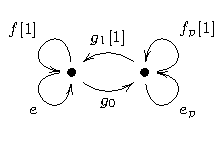
\includegraphics[width=0.26\linewidth]{figures/quiver.pdf}
\end{center}

本节余下部分概述如何建立下述结果：

\begin{proposition}\label{prop:6.2}
在上述记号下，有
\[
HH^{d,2-d}(Q)=\begin{cases}k, & d=6,8,\\ 0, & d>2,\ d\neq6,8.\end{cases}
\]
\end{proposition}

在此之前，我们先说明下述重要推论，它是整个计算的动机。该推论把我们的 Hochschild 上同调计算的含义明确写出，所用工具是定理 \ref{thm:5.3} 关于 Hochschild 上同调与 $A_\infty$-结构关系的理论，连同定理 \ref{thm:2.1} 的同调微扰论。

\begin{corollary*}
每个满足 $H(\mathcal{Q}')\simeq Q$ 的 $A_\infty$-代数 $(\mathcal{Q}',m_d)$ 都拟同构于一个极小 $A_\infty$-代数 $(\tilde{\mathcal{Q}},\tilde m_d)$，使得 $\tilde m_d=0$ 对 $d\le5$ 或 $d=7$。结构映射 $\tilde m_6$ 与 $\tilde m_8$ 在 $HH^{6,-4}(A)$ 与 $HH^{8,-6}(A)$ 中定义上链。

此外，若 $(\mathcal{Q}',m_d)$ 与 $(\mathcal{Q}'',m'_d)$ 是如上两个极小 $A_\infty$-代数，且 $[m_6]=[m'_6]$、$[m_8]=[m'_8]$，则 $\mathcal{Q}'$ 与 $\mathcal{Q}''$ 规范等价。

特别地，$Q$ 上 $A_\infty$-结构在拟同构意义下的空间至多是一维的。
\end{corollary*}

% [Tutor Note: 原文疑误：推论中写 $HH^{6,-4}(A)$ 与 $HH^{8,-6}(A)$，但本推论讨论的是 $Q$ 上的 $A_\infty$-结构，应为 $HH^{6,-4}(Q)$ 与 $HH^{8,-6}(Q)$（与 p.25 及命题 6.2 的写法一致）。译文保留原文写法。]

% [Tutor Note: 推论中“极小”指 $m_1=0$；homological perturbation 保证任何 $A_\infty$-代数都拟同构于极小的一个。注意 $m_6$ 与 $m_8$ 分别对应 $HH^{6,-4}$ 与 $HH^{8,-6}$：$m_d$ 的次数为 $2-d$，故落在第二个指标 $2-d$ 上，这不是笔误。]

证明的出发点是观察 $HH^{m,n}(A)=\Ext^m_{A\otimes A^{op}}(A,A(n))$（见第 \ref{subsec:hoch-cohomology} 小节）。因此，可以通过为有限维分次代数 $Q^e=Q\otimes Q^{op}$ 找到一个显式的投射消解来建立该定理。这看起来相当没有启发性。所以我们先看看用更抽象的论证能得到什么。

现在的关键观察是：$Q$ 是域上的有限维代数。这开启了一大套一般理论，参见例如 [22]。（该文献处理的是未分次的代数与模，但到分次情形的改造是直接的。）

$Q$ 的极小幂等元是 $e_1=e$ 与 $e_2=e_p$。由此可知 $P_i=Qe_i$（$i=1,2$）是极小不可分解投射 $Q$-模，且所有这些模都具有 $P_i(n)$ 的形式（对某个 $n$）。这些投射模有唯一的非平凡单商模 $S_i$，而这样我们就再次得到全部单 $Q$-模。事实上，$S_i$ 是一维 $k$-向量空间，分别由 $e$ 与 $e_p$ 的类张成。

由一般理论可知，$Q^e$ 的极小投射模是 $P_{ij}(m)=(e_iQe_j)(m)$，单模是 $S_{ij}(m)=\Hom_k(S_i,S_j)(m)$。于是，把 [7] 中引理 1.5 的论证改造到分次情形，我们得到：

\begin{lemma*}
设 $\cdots\to R_n\to R_{n-1}\to\cdots\to R_1\to R_0\to Q$ 是 $Q$ 作为 $Q^e$-模的极小投射消解。则
\[
R_n=\bigoplus_{i,j,m}P_{i,j}(m)^{\Ext^n_Q(S_i,S_j(m))}.
\]
\end{lemma*}

现在容易验证存在正合列
\begin{gather*}
0\longleftarrow S_1\longleftarrow P_1\xleftarrow{\ \times g_0\ }P_1\xleftarrow{\ \times f_p\ }S_2(-1)\longleftarrow 0\\
0\longleftarrow S_2\longleftarrow P_2\xleftarrow{\ \times g_1\ }P_2(-1)\xleftarrow{\ \times f\ }S_1(-2)\longleftarrow 0
\end{gather*}
从而存在如下投射消解：
\begin{gather*}
\cdots\to P_1(-3)\to P_1(-3)\xrightarrow{\ \cdot\ }P_2(-2)\to P_2(-1)\to P_1\to P_1\to S_1\to 0\\
\cdots\to P_2(-4)\to P_2(-3)\xrightarrow{\ \cdot\ }P_1(-2)\to P_1(-2)\to P_2(-1)\to P_2\to S_2\to 0
\end{gather*}
忽略分次后，这些消解以四为周期。带点的箭头表示第一个周期的结束；当然，末尾的 $S_i\to0$ 部分不重复。经过每个周期后，分次增加三。

% [Tutor Note: 核对要点：两个短正合列并不对称——第一列是 $S_1\leftarrow P_1\leftarrow P_1\leftarrow S_2(-1)$（第二个 $P_1$ 无平移），第二列是 $S_2\leftarrow P_2\leftarrow P_2(-1)\leftarrow S_1(-2)$。“无平移”与“$(-1)$”的差别正是把 $S_2(-1)$、$S_1(-2)$ 逐步代换、拼出周期消解的关键；抄写时不要“顺手补齐对称性”。]

% [Tutor Note: 消解中的映射都是左乘相应元素（$\times g_0$、$\times f_p$ 等）。带点箭头的“周期”是：$S_1$ 的消解由 $S_2(-1)$ 的消解接续，而 $S_2(-1)$ 的消解又由 $S_1(-3)$ 的消解接续，如此循环，每循环一次整体平移 $-3$，故“分次增加三”。]

现在注意到 $\Hom_Q(P_i(n),S_j(m))=\Hom_Q(S_i(n),S_j(m))$ 在 $i=j=n=m$ 之外为零，于是由引理推出：类似地，$Q$ 在 $Q^e$ 上有一个投射消解，忽略分次时以八为周期，且经过每个周期后分次增加六。

特别地，由此可知对任意 $l$，当 $n$ 充分大时 $HH^{n,l-n}(Q)=0$。事实上，它是 $\Hom_{Q^e}(R_n,Q(l-n))=\Hom_{Q^e}(R_n([6n/8]),Q(l-n+[6n/8]))$ 的一个子商，而由消解的周期性，$R_n([6n/8])$ 只依赖于 $n\pmod 8$，同时 $Q(l-n+[6n/8])$ 终将落在任意高的次数上。这里 $[x]$ 表示不超过 $x$ 的最大整数。

% [Tutor Note: 注意第二个指标：前一句用一般参数 $l$（即 $HH^{n,l-n}$），后一句取 $l=2$（即 $HH^{n,2-n}$），因为 $A_\infty$-结构的形变方向是 $HH^{\bullet,2-\bullet}$（$m_d$ 的次数为 $2-d$）。这是本页最易混的下标，命题 6.2 与推论的指标都由它决定。]

更仔细一些，容易确切找出极小投射消解中出现的模，并给出使 $HH^{n,2-n}=0$ 成立的 $n$ 的显式下界。于是证明该命题就只剩两件事：把 $Q$ 的投射消解具体算到有限长度（例如真正确定消解中模之间的映射），并计算低维 Hochschild 上同调。这是件苦差事，最好交给计算机。若有特别受虐狂的读者想手工验证，她会受益于这样一个事实：不仅极小投射消解中的模是周期的，映射也是周期的。因此整个命题可以通过找出这个周期消解来建立。详细计算已在 [12, 定理 4] 中完成。

该命题也在 [11] 中用（不同的）方法重新证明过。

% [Tutor Note: 作者省略的全部计算是：$Q$ 的极小投射消解周期为 8、映射亦周期（正文明说），因此只需把前 8 步的映射矩阵写出、并对 $n=0,\dots,7$ 计算 $\Ext^n$；$HH^{d,2-d}=k$ 只在 $d=6,8$ 出现，正好解释了为什么只有 $m_6,m_8$ 无法被平凡化。可用矩阵模型 $Q\subset M_2(k[s]/s^2)$ 手算，或按 [12] 的程序实现。]
